\documentclass[twoside,11pt]{article}

% Any additional packages needed should be included after jmlr2e.
% Note that jmlr2e.sty includes epsfig, amssymb, natbib and graphicx,
% and defines many common macros, such as 'proof' and 'example'.
%
% It also sets the bibliographystyle to plainnat; for more information on
% natbib citation styles, see the natbib documentation, a copy of which
% is archived at http://www.jmlr.org/format/natbib.pdf

\usepackage{csc498project}
\usepackage{graphicx}
\usepackage{hyperref}
\usepackage{listings}
% Python code color format
% Source: https://www.overleaf.com/learn/latex/Code_listing
\usepackage{xcolor}

\definecolor{codegreen}{rgb}{0,0.6,0}
\definecolor{codegray}{rgb}{0.5,0.5,0.5}
\definecolor{codepurple}{rgb}{0.58,0,0.82}
\definecolor{backcolour}{rgb}{0.95,0.95,0.92}

\lstdefinestyle{mystyle}{
    backgroundcolor=\color{backcolour},   
    commentstyle=\color{codegreen},
    keywordstyle=\color{magenta},
    numberstyle=\tiny\color{codegray},
    stringstyle=\color{codepurple},
    basicstyle=\ttfamily\footnotesize,
    breakatwhitespace=false,         
    breaklines=true,                 
    captionpos=b,                    
    keepspaces=true,                 
    numbers=left,                    
    numbersep=5pt,                  
    showspaces=false,                
    showstringspaces=false,
    showtabs=false,                  
    tabsize=2
}

\lstset{style=mystyle}
\graphicspath{ {./images/} }
% Short headings should be running head and authors last names

\ShortHeadings{Sokoban RL}{Deval Patel, Kyrel Jerome}
\firstpageno{1}


\title{Sokoban RL}

\author{\name Deval Patel \email devalm.patel@mail.utoronto.ca \\
       \addr 1005468655\\
       \AND
      \name Kyrel Jerome \email kyrel.jerome@mail.utoronto.ca \\
       \addr 1004186169}

\begin{document}

\maketitle

\begin{abstract}%   <- trailing '%' for backward compatibility of .sty file
We proceed to implement a custom Sokoban environment using OpenAI Gym's custom environment feature. To test our environment, we use Stable Baselines 3 algorithms, particularly A2C, DQN and PPO. We experimented with different levels as well as reward schemes.
\end{abstract}

\section{Introduction}
Our project creates a custom RL environment based off of the puzzle game Sokoban. Then we proceed to test our environment on 3 state of the art algorithms; A2C, DQN and PPO. We will talk more about them later in this report. Our project's repository can be found at \url{https://github.com/deval-patel/sokobanRL}.

Our original idea for the project was to have 2 RL agents, where one would learn how to solve the puzzle, and the other would be able to learn how to \textit{create} new puzzles. However, it was deemed out of scope, so we did not end up doing PCGRL based on the paper by \cite{khalifa2020pcgrl}

Instead, as a TA suggested we make our own environment and analyze it with different algorithms. 

\subsection{What is Sokoban?}
Sokoban is a grid-based single player puzzle game of Japanese origins where the player must make movements in one of the 4 cardinal directions throughout the game to cover checkpoints with boxes by pushing the boxes onto the checkpoints \cite{sokoban_wiki}. This is the basics of the game, however there is often a turn limit associated with a level. This means that in a certain number of turns, the player must solve the level otherwise they lose. Another alternative approach is a push limit. This limits the number of times they are allowed to push a box. Both of these constraints adds an extra difficulty to the simple puzzle solving game, making the problem of solving Sokoban Levels an NP Hard problem.
\begin{figure}[h]
       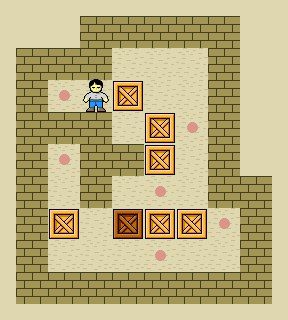
\includegraphics[scale=0.5]{default_map-0.png}   
       \centering    
       \caption{Sample Sokoban Map}
\end{figure}

\section{Environment}
As mentioned previously, we made our own custom RL environment. In order to do this, we had to first make the game itself. The code is quite modular following good software design principals and can be found at \verb|sokobanRL/gym\_498\_sokoban|. The main game logic is found in \verb|sokobanRL/gym_498_sokoban/SokobanGame.py|. To run the game in text format, you can run 
\verb|sokobanRL/gym_498_sokoban/SokobanController.py|. 

\subsection{Creating Custom Gym Environment}
We used OpenAI Gym's environment creation guide in order to create our custom gym environment \cite{openai_2021}. We chose to do this as OpenAI's gym provides a good template for environment code and it was easy to pick up. Furthermore, we ended up using \cite{stable-baselines3} which contains implementations of state of the art algorithms in order to test our environment. The good thing about stable baselines3 is its support for gym environments. Our custom gym environments can be found under \verb|sokobanRL/gym_498_sokoban/envs/|.

\subsubsection{Observation Space}
Our observation space is a Box of type \verb|np.uint8|. We pass in the state of the grid to the agent as an observation. Therefore, we used a Box with the shape of the grid (\verb|shape=(height, width)|). We also set $low=0$ and $high=6$ limits on the values of our box since that represents the unique pieces we have for our game.

\noindent\textbf{Pieces Mapping:}\\
\begin{lstlisting}[language=Python]
EMPTY: int = 0
WALL: int = 1
TARGET: int = 2
BOX: int = 3
BOX_ON_TARGET: int = 4
PLAYER: int = 5
PLAYER_ON_TARGET: int = 6
\end{lstlisting}

\subsubsection{Action Space}
Our action space is discrete and of size 4. The agent is able to move the player in one of the 4 cardinal directions, UP, DOWN, LEFT or RIGHT. Each of these actions are mapped to integers, which resulted in our discrete action space.

\subsubsection{Transitions}
Depending on the action that the agent chooses, a move corresponding to that action will be made (moving the player in the direction of the action, if valid). The algorithm can be summarized in the following steps (can be found under \verb|sokobanRL/gym_498_sokoban/SokobanGame.py:132|). 

\begin{enumerate}
       \item Check for a valid move given an action.
       \item Store current state in stack
       \item Check if the action requires a box to be pushed. If so, move the box.
       \item Move the player to their new position.
       \item Decrement the turn limit by 1 since a succesful turn has been made.
       \item Return the reward based on the move.
\end{enumerate}

\subsubsection{Rewards}
Reinforcement Learning is based on the idea of an agent maximizing the reward it can achieve. As a result, the agent needs to be awarded for making actions in our environment. We define the following reward system (\verb|sokobanRL/gym_498_sokoban/RewardSystem.py|):\\

\noindent\textbf{Reward for Move (no effect):} $-0.05$\\
This is a slight negative reward for making any move. We provide a slight negative reward so that the agent does not make unnecessary moves, since turn limit is an optional factor in the game as well. We want the agent to win in the optimal number of turns.\\\\
\textbf{Reward for Invalid Move:} $-3.0$\\
If the agent takes an action which makes them move the player into the wall or into a box which cannot be pushed, they receive a slightly higher negative reward since this move does not do anything productive.\\\\
\textbf{Reward for Moving Box on Target:} $8.0$
We reward the agent positively for moving the boxes onto the target, as this is a part of the win condition. Remember, to win this puzzle game, the agent is required to move all boxes onto the targets.\\\\
\textbf{Reward for Moving Box off Target:} $-8.0$\\
On the other hand, if the agent moves a box off of a target, then this is likely going against the win condition, so we penalize the agent to avoid this mistake.\\\\
\textbf{Reward for Victory:} $30.0$\\
Finally, if the agent completes the level, they are rewarded with a largely positive reward.\\\\
\textbf{Reward for Loss:} $-30.0$\\
If the agent is to lose the game, they are penalized with a largely negative reward.

\section{Algorithms}
For our algorithms, we used Stable Baselines3 as it contains stable implementations of state of the art algorithms. Although SB3 has 7 RL algorithms at its disposal (A2C, DDPG, DQN, HER, PPO, SAC, TD3) we were limited to using A2C, DQN and PPO. This is because the algorithms use case is limited on the action and observation spaces. Since we have a discrete action space and a box observation space, we could not use DDPG, SAC and TD3. A2C and DQN were covered in this courses' material, however PPO was not and we were excited to use a new algorithm and explore its performance.

\begin{figure}[h]
       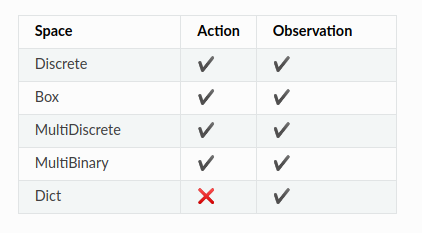
\includegraphics[scale=0.75]{a2c_use.png}   
       \centering    
       \caption{A2C Use Cases}
\end{figure}

\subsection{A2C}
Advantage Actor Critic as learned in lecture uses 2 models (the actor and critic). The actor learns the policy, whereas the critic evaluates our actions and acts as our value function. The implementation that SB3 uses (ACKTR: Actor Critic using Kronecker-factored Trust Region) combines three techniques: actor-critic methods, trust region optmization and distributed Kronecker factorization \cite{wu_2020}. ACKTR takes a step in the \textit{natural gradient} instead of the gradient direction. As we learned in class, limiting the KL divergence helps with consistency, so that our policy does not drastically change on an update (this could lead to worse performance). 
\subsection{DQN}
Deep Q-Learning learns Q values with a neural network. As we learned in class, there are several hyperparameters which can be configured for DQN and there are also algorithmic variants which build on the fundamentals that DQN has set. Since DQN can succesfully perform with high dimension inputs, it was a good option for our environment \cite{mnih2015human}. SB3's implementation of DQN builds on Fitted Q-Iteration (FQI) and uses tricks for stable learning with the neural network. It uses a replay buffer, a target network as well as gradient clipping \cite{stable-baselines3}. The implementation is just a vanilla DQN, there is no further support for Double-DQN, Dueling-DQN or Prioritized Experience Replay. This was unfortunate as we wished to experiment with further optimizations of DQN that we learned and implemented in the course.
\subsection{PPO}
Proximal Policy Optimization is an algorithm that was not covered in this course. The algorithm combines ideas from A2C such as having multiple workers and it also uses a trust region to improve the actor. When PPO makes an update for its policy, the new policy should not be \textit{too far} from the old policy. Similarly to ACKTR, PPO uses clipping in order to avoid too large of an update. Furthermore, the advantages computed are normalized and the critic can also be clipped. These are some further modifications made by OpenAI compared to the original paper on PPO by \cite{schulman2017proximal}.

Something that we found interesting is that SB3's new PPO algorithm does not use an adaptive KL penalty. It uses a different objective function which is not common in other algorithms. This makes the algorithm simpler and removes adaptive updates. However, it matches ACER's (Actor Critic with Experience Replay) performance despite being simpler to implement.

\begin{figure}[h]
       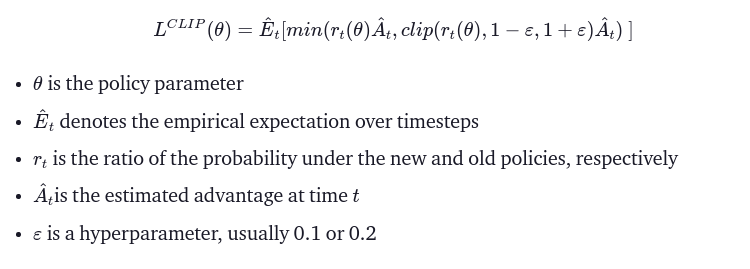
\includegraphics[scale=0.5]{trust_region_update.png}   
       \centering    
       \caption{Trust Region Update \cite{schulman_2020}}
\end{figure}

\section{Experiments}
To enable the use of the above algorithms we implemented sets of generalized classes around the Stable Baselines engine. The classes enabled us to interchangeably interact with and design constraints for the individual agents. To enable the Stable Baselines framework to properly interact with the sokoban environment, we created a Solid Baselines Custom Environment such that the agents and pre-built algorithms can properly interact with the environment.

Due to time constraints along with issues interacting with the Stable Baselines logging interface, we were unable to complete our assessment of which algorithms perform best on a multitude of maps. Our goal for evaluation was to first generate and train a learning agent on the training maps, with the hope that the agent would diversify to function on the validation and test maps.

To further test the agents, our goal was to test using differing sets of hyper-parameters along with neural network sizes. In the future, we would choose to select the bot during training that best functions on the validation test set, allowing us to ensure that the model is not over-fitting to the training maps.

\section{Conclusion}
By implementing a custom RL environment for Sokoban, our work provides the required base for multiple further environment projects. Specifically, in later projects this implementation may be used to explore the use of machine learning agents to procedurally generate levels, using a pre-trained agent to determine the viability or difficulty of the output levels. In its current state, our project presents a platform and tooling to assess the functionality of discrete action machine learning algorithms on the Sokoban game.


% Manual newpage inserted to improve layout of sample file - not
% needed in general before appendices/bibliography.

\bibliography{bibliography}

\end{document}